% CHAPTER 2

\chapter{UAV}\label{ch:uav}
Un aeromobile a pilotaggio remoto (\acs{UAV}) è un velivolo caratterizzato dall'assenza di un pilota umano a bordo. Il suo volo può essere controllato da un computer a bordo del mezzo oppure da remoto, seguendo i comandi di un pilota a terra.

% ------------------------------ CLASSIFICAZIONE ------------------------------

\section{Classificazione}
In base al numero e alla configurazione dei rotori si possono distinguere diverse tipologie di droni \cite{droneClass}, come mostrato in Figura \ref{fig:droneTypes}.\\

Il modello di drone più semplice è quello a singolo rotore. Presenta un solo rotore al suo interno e un secondo rotore di coda necessario per fornire il controllo. Questo modello si rivela un'ottima soluzione nel caso si debba trasportare dei carichi particolarmente pesanti per un breve tempo di volo.\\

Aumentando il numero di eliche a tre e disponendole in modo da formare una Y, si ottiene la configurazione del tricopter. Questo è costituito da tre motori, tre controllori, quattro giroscopi e un servomotore. I motori sono posizionati alle estremità dei tre bracci e ognuno presenta un sensore di posizione. È in grado di rimanere stabile lungo un determinato percorso grazie ai sensori di posizione e non necessita di correzione manuale.\\

La configurazione più diffusa è quella a quattro eliche, che caratterizza la tipologia del quadrirotore (quadcopter). Le quattro eliche possono assumere la disposizione a + (QUAD I) oppure a X (QUAD X), come mostra Figura \ref{fig:droneTypes}.\\

Esistono anche configurazioni a sei e otto rotori. Queste configurazioni sono sicuramente più stabili rispetto a quelle con un numero minore di eliche e consentono inoltre di controllare il velivolo con più precisione.

\begin{figure}[H]
    \centering
    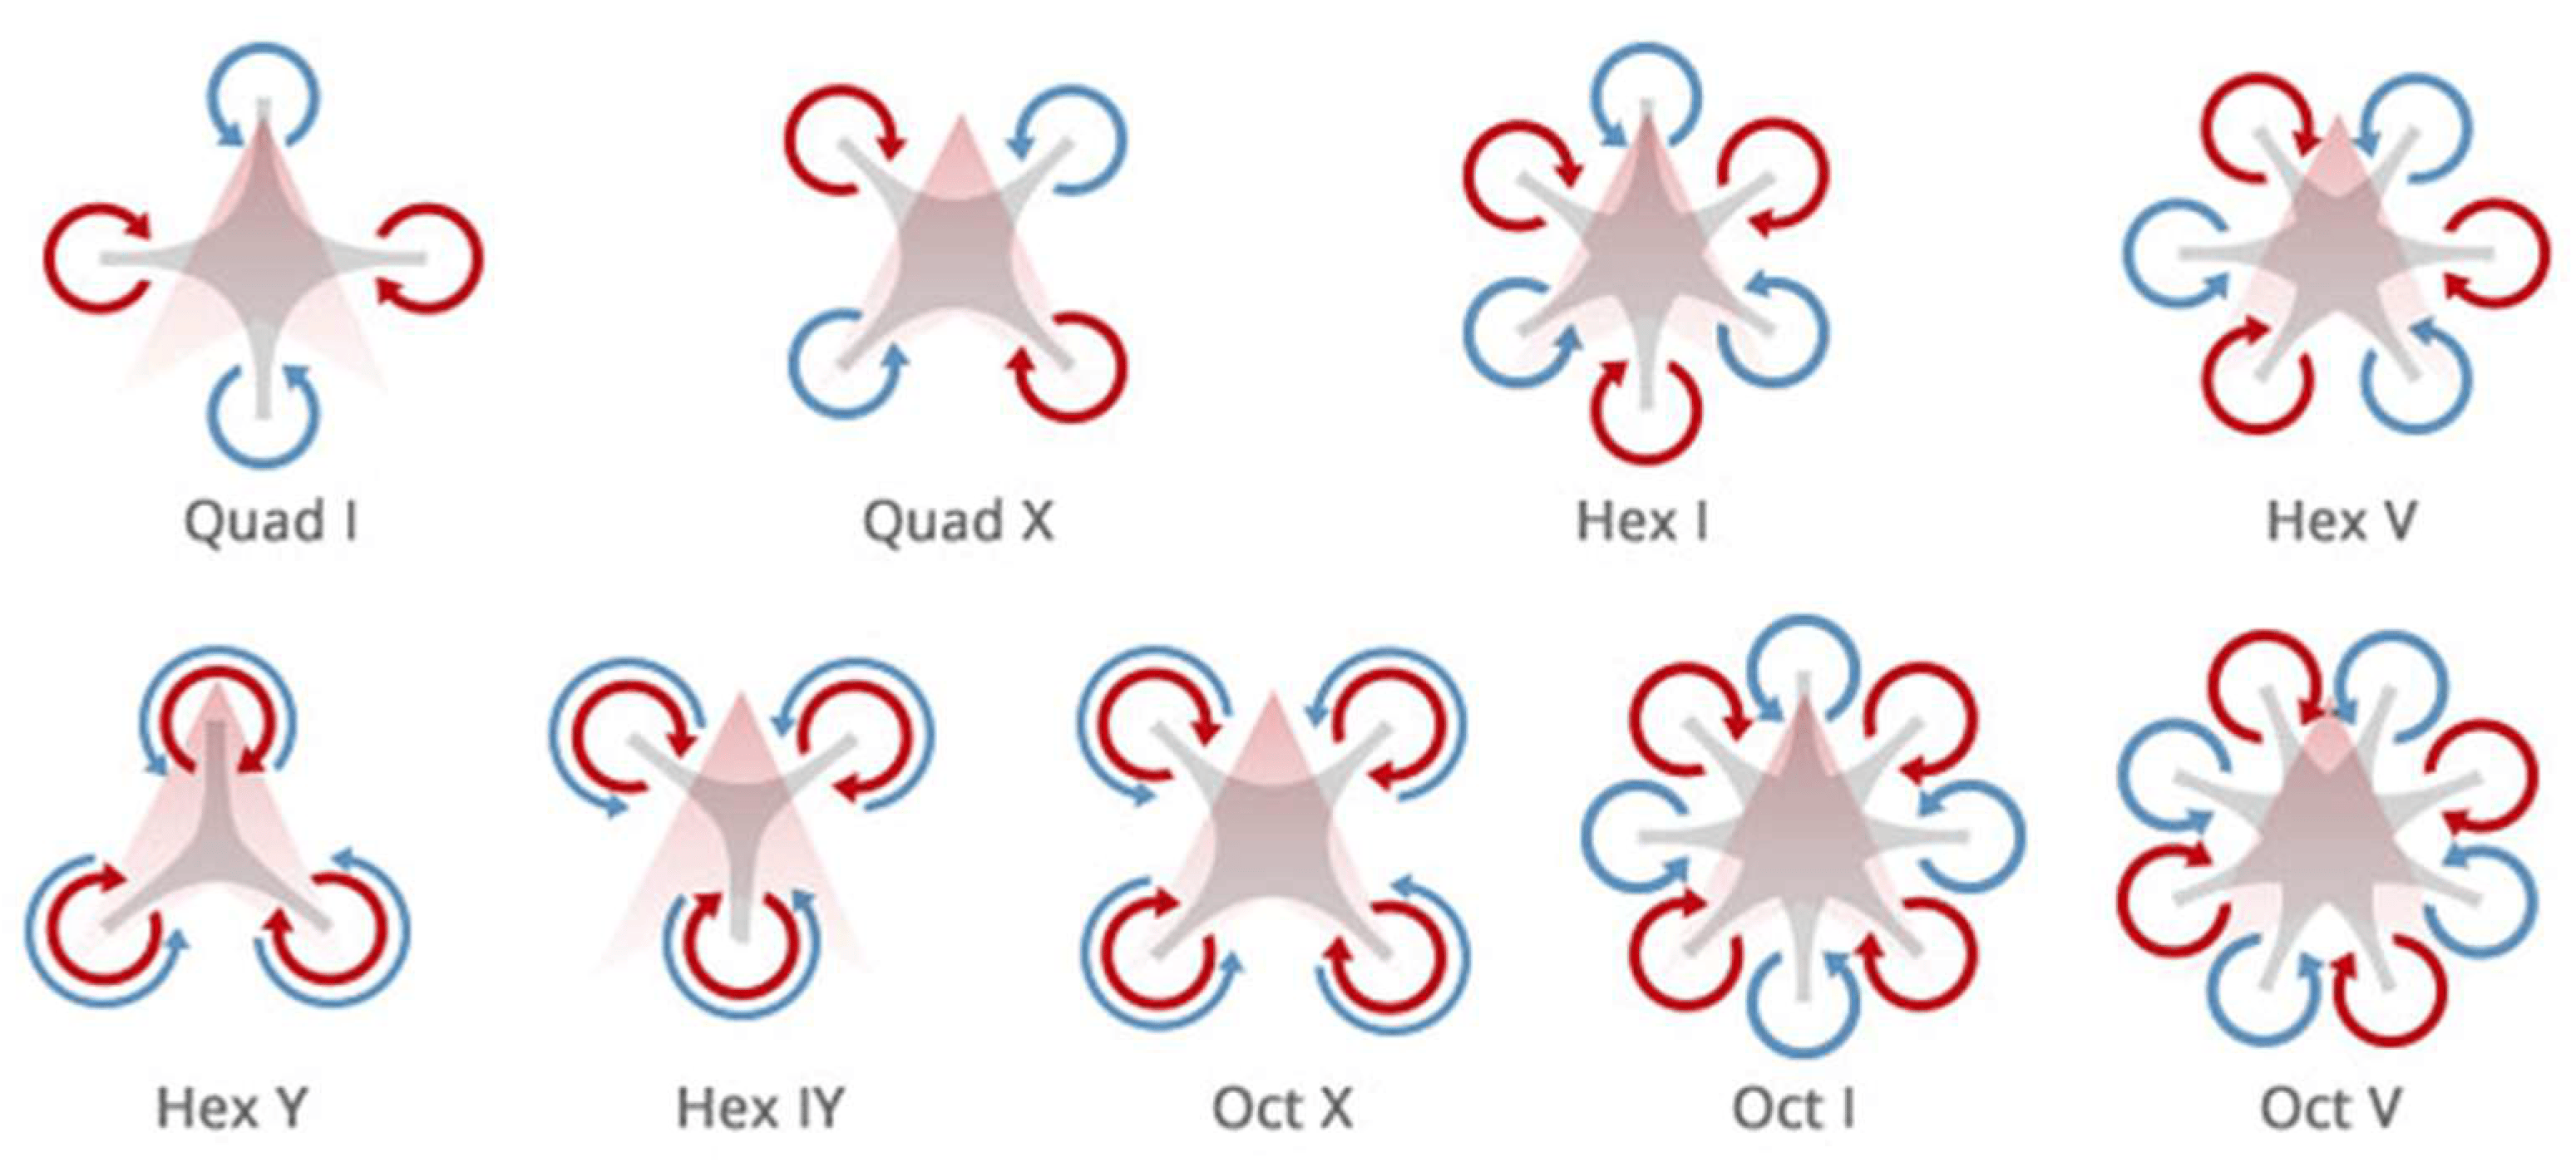
\includegraphics[width=0.75\textwidth]{gfx/drone_types}
    \caption[Classificazione multi-rotori.]{Classificazione multi-rotori in base al numero e alla configurazione dei rotori.}
    \label{fig:droneTypes}
\end{figure}

Nel seguito si prenderà come riferimento un quadrirotore con struttura a X dato che presenta un modello fisico-matematico semplificato e rende pertanto più semplice il progetto di schemi di controllo e l'identificazione del sistema. Inoltre, questa disposizione dei rotori minimizza la variazione di posizione del baricentro e risulta pertanto più semplice tenere traccia della traiettoria del drone nello spazio.

% ------------------------------ MODELLAZIONE ------------------------------

\section{Modellazione Matematica di un Quadrirotore}
Un robot, nello specifico un quadrirotore, può essere considerato come un corpo rigido che trasla e ruota in uno spazio tridimensionale. Pertanto, è necessario costruire un modello matematico in grado di descrivere in modo compatto il suo spostamento.\\

Il modello fisico-matematico di un quadrirotore si può trovare con diversi formalismi, quali quello di Newton-Eulero e quello di Lagrange \cite{modelloQuad1} \cite{modelloQuad2} \cite{modelloQuad3}. Nel seguito si descrive il primo.\\

Nello specifico, si tratta di un sistema a sei gradi di libertà - 6 \ac{DoF} - quindi è descrivibile utilizzando dodici stati\footnote{Per ogni grado di libertà si considerano due stati: uno descrive la variabile considerata in un determinato istante di tempo $t$, l'altro ne descrive l'evoluzione nel tempo. Nel caso di un sistema tempo discreto è sufficiente calcolare la variabile nell'istante discreto successivo $t + T_C$, dove $T_C$ è il periodo di campionamento (Metodo Differenze Finite). Siccome $T_C$ è un tempo costante si può normalizzare il periodo di campionamento rendendolo unitario. Nel caso di un sistema tempo continuo si estende lo stesso ragionamento tramite l'operatore di derivata (Metodo Eulero). Se ad esempio la variabile considerata rappresenta una posizione, la sua evoluzione è una velocità.}: sei per la posizione, sei per l'assetto. Il sistema pertanto risulta sotto-attuato perché è caratterizzato da sei gradi di libertà, ma il suo movimento nello spazio può essere controllato soltanto da quattro attuatori (uno per ogni elica). In particolare, variando le velocità angolari delle eliche del velivolo è possibile effettuare tutti i movimenti.

\begin{figure}[H]
    \centering
    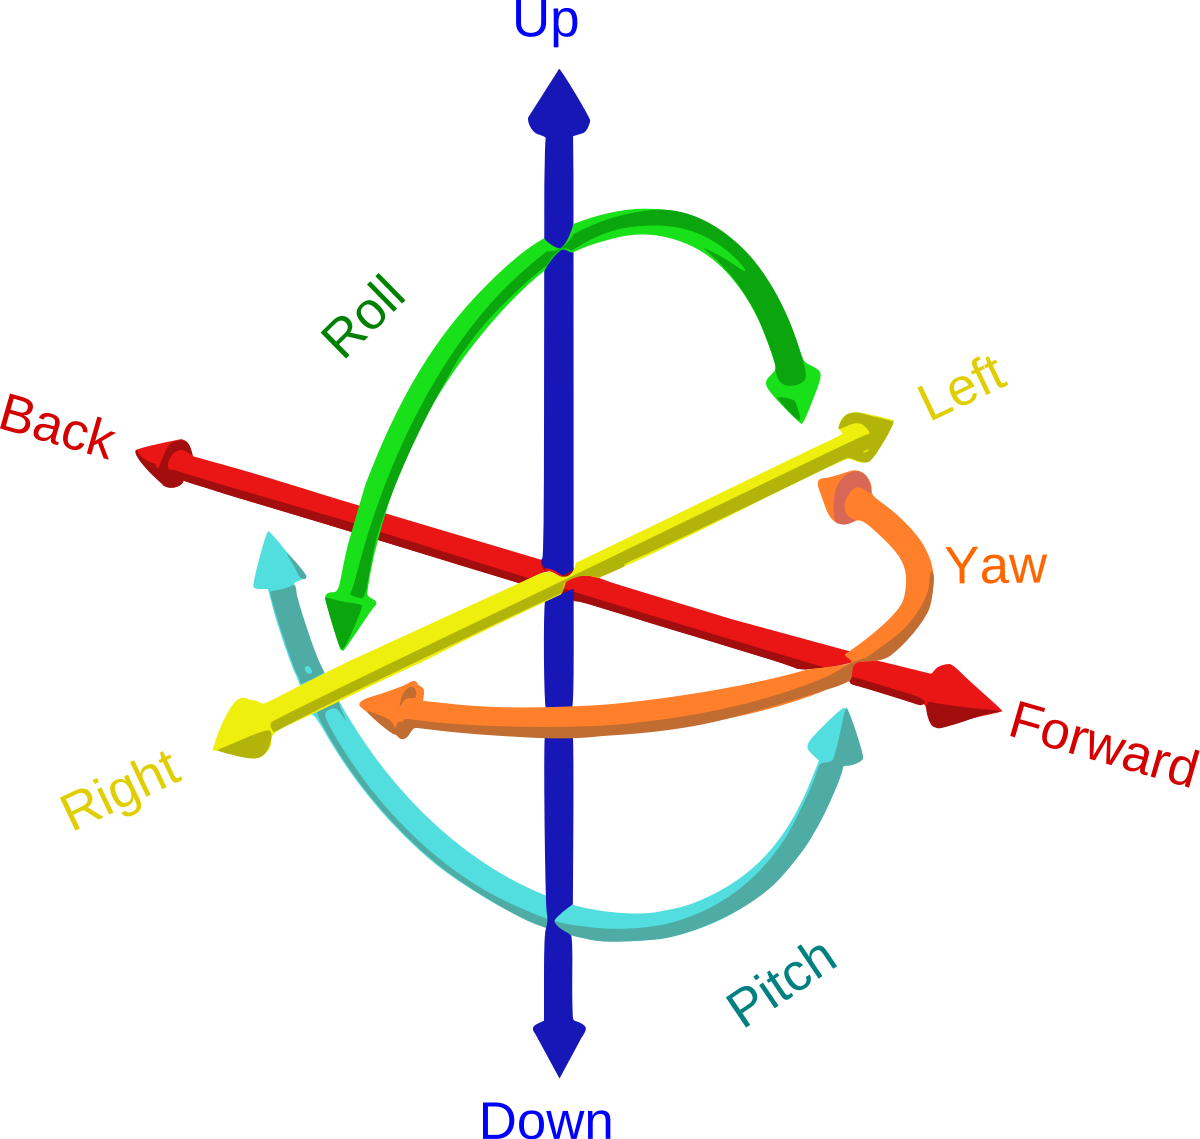
\includegraphics[width=0.3\textwidth]{gfx/6dof}
    \caption[Sei gradi di libertà (6 \acs{DoF}) di un corpo rigido in uno spazio tridimensionale.]{Sei gradi di libertà (6 \acs{DoF}) di un corpo rigido in uno spazio tridimensionale.}
\end{figure}

\subsection{Sistemi di Riferimento}

Prima di poter descrivere le equazioni che governano un velivolo, come il quadrirotore, è necessario definire le coordinate di riferimento in cui si intende farlo. Sono necessari due sistemi di riferimento per descrivere la posizione e l'assetto del drone nello spazio: un sistema \emph{mondo} (earth frame o $E$) inerziale, e un sistema \emph{drone} (body frame o $B$) solidale al velivolo in movimento, le cui dinamiche possono essere espresse rispetto alla terna fissa. La terna fissa (inerziale) è una terna dove si può considerare valida la prima legge di Newton.\\

Il sistema \emph{mondo} può essere definito secondo le coordinate \ac{LTP}, relative al piano tangente ad ogni punto della superficie terrestre. Esistono due convenzioni: il sistema \ac{ENU} è definito da una terna i cui versori sono orientati verso Est, Nord (piano tangente) e verso l'esterno della terra (Figura \ref{fig:fixedRef}), il sistema \ac{NED} è definito analogamente con Est e Nord scambiati e punta verso l'interno della terra.

\begin{figure}[H]
    \centering
    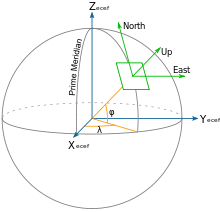
\includegraphics[width=0.29\textwidth]{gfx/ltp_enu}
    \caption[Sistema di riferimento \acs{ENU}.]{Sistema di riferimento \acs{ENU}, tangente alla superficie terrestre.}
    \label{fig:fixedRef}
\end{figure}

Il sistema \emph{drone} ha origine nel centro di massa del quadrirotore e in letteratura viene definito come \ac{ABC}. Questa terna mobile varia a seconda della configurazione dei rotori del quadrirotore, come mostra Figura \ref{fig:+andx}. Nel caso di un quadrirotore con disposizione a + si considerano gli assi x e y coincidenti con i due assi principali del quadrirotore. Nel caso in oggetto (disposizione a X), invece, gli assi x e y corrispondono alle bisettrici dei due assi principali del quadrirotore.

\begin{figure}[H]
    \centering
    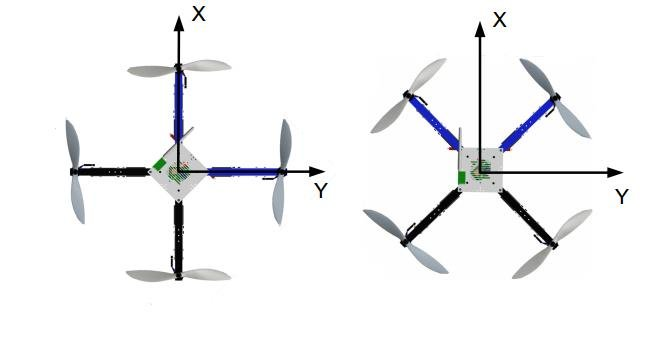
\includegraphics[width=0.53\textwidth]{gfx/+andx}
    \caption[\acs{ABC} di un QUAD I e di un QUAD X.]{\acs{ABC} di un QUAD I e di un QUAD X.}
    \label{fig:+andx}
\end{figure}

Figura \ref{fig:abc_frame} presenta i due sistemi di riferimento \emph{mondo} e \emph{drone}, secondo le ipotesi formulate.

\begin{figure}[H]
    \centering
    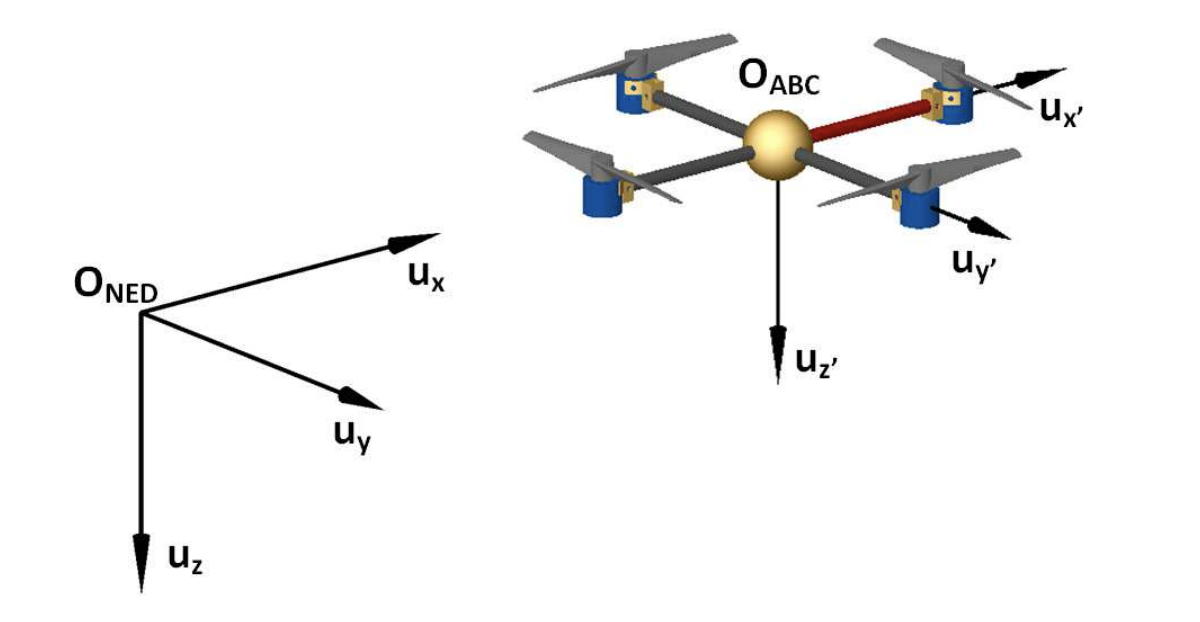
\includegraphics[width=0.7\textwidth]{gfx/abc_frame}
    \caption[Sistemi di riferimento \acs{NED} e \acs{ABC}.]{Sistemi di riferimento \acs{NED} e \acs{ABC}, utilizzati nella modellazione di un quadrirotore.}
    \label{fig:abc_frame}
\end{figure}

\subsection{Trasformazioni}

Dato che il drone trasla e ruota, è necessario stabilire per entrambi i moti un modo per poter passare dal sistema di riferimento \emph{mondo} al sistema di riferimento \emph{drone} e viceversa. 

\section*{Traslazioni}
Per le traslazioni è sufficiente utilizzare la somma vettoriale nello spazio a tre dimensioni di riferimento. Infatti, dato un generico punto $P$ rappresentato nel sistema di riferimento del velivolo $O_{ABC}$ dal vettore $v^P_{ABC}$, esiste un vettore di traslazione che permette di rappresentare lo stesso punto nel sistema di riferimento a terra. Nello specifico:
\[ v^p_{NED} = v^p_{ABC} + t_{NED} \]
dove $v^P_{NED}$ è il vettore che rappresenta il punto $P$ nel sistema di riferimento a terra e $t_{NED}$ è il vettore di traslazione. 

\section*{Rotazioni}
Le rotazioni possono essere descritte assumendo il corpo rigido fisso (in termini di posizione) nell'origine di un sistema di riferimento, con i tre versori del sistema che cambiano sotto l'effetto di rotazioni. Quindi, la rotazione è una relazione tra un sistema di riferimento fisso e lo stesso sistema (cioè con stessa origine) ruotato rispetto ai tre angoli di Eulero (cioè rispetto ai tre assi). La rotazione di un angolo intorno ad un asse può essere rappresentata da una matrice le cui colonne corrispondono ai versori del sistema ruotato. Considerando i tre possibili angoli di rotazione relativi ai tre assi del sistema di riferimento, si ottengono le seguenti tre matrici di rotazione ortonormali, cioè tali che $R^\top = R^{-1}$.

\begin{itemize}
	\item Rotazione intorno all'asse x:
	\begin{equation}
	R_x(\phi) = 
	\begin{bmatrix}
		1 & 0 & 0\\
		0 & \cos(\phi) & \sin(\phi)\\
		0 & -\sin(\phi) & \cos(\phi)
	\end{bmatrix}
	\end{equation}
	\item Rotazione intorno all'asse y:
	\begin{equation}
	R_y(\theta) = 
	\begin{bmatrix}
		\cos(\theta) & 0 & \sin(\theta)\\
		0 & 1 & 0\\
		-\sin(\theta) & 0 & \cos(\theta)
	\end{bmatrix}
	\end{equation}
	\item Rotazione introno all'asse z:
	\begin{equation}
	R_z(\psi) = 
	\begin{bmatrix}
		\cos(\psi) & \sin(\psi) & 0\\
		-\sin(\psi) & \cos(\psi) & 0\\
		0 & 0 & 1
	\end{bmatrix}
	\end{equation}
\end{itemize}

Quindi, dato un generico punto $P$ rappresentato nel sistema di riferimento traslato ma non ruotato $O_{xyz}$ dal vettore $v^P_{xyz}$, la trasformazione che consente di rappresentare lo stesso punto nel sistema di riferimento $O_{x'y'z'}$ ruotato intorno all'origine rispetto ad uno specifico asse (e.g. asse x) è la seguente:
\[ v^P_{x'y'z'} =  R_x(\bar{\phi})v^P_{xyz}\]
dove $v^P_{x'y'z'}$ è il vettore che rappresenta $P$ nel sistema ruotato intorno all'asse x di un angolo $\bar{\phi}$, come indicato nella matrice di rotazione.\\

A questo punto, si definisce la \ac{DCM} come il prodotto delle tre matrici di rotazione per passare da un sistema di riferimento all'altro. Per semplificare la notazione, le funzioni trigonometriche  $\sin (\cdot)$ e $\cos (\cdot)$ sono talvolta indicate come $s(\cdot)$ e $c(\cdot)$, rispettivamente.\\

Per passare dal sistema \emph{mondo} al sistema \emph{drone} si considera la seguente matrice di trasformazione:
\[
R_{EB}(\phi,\theta,\psi) = 
R_x(\phi)R_y(\theta)R_z(\psi) = 
\]
\begin{equation}
=
\begin{bmatrix}
c(\theta)c(\psi) & c(\theta)s(\psi) & -s(\theta)\\
s(\phi)s(\theta)c(\psi)-c(\phi)s(\psi) & s(\phi)s(\theta)c(\psi)+c(\phi)c(\psi) & s(\phi)c(\theta)\\
c(\phi)s(\theta)c(\psi)+s(\phi)s(\psi) & c(\phi)s(\theta)s(\psi)-s(\phi)c(\psi) & c(\phi)c(\theta)
\end{bmatrix}
\label{dcmEB}
\end{equation}

Per passare dal sistema \emph{drone} al sistema \emph{mondo}, invece, si considera la seguente matrice di trasformazione:
\[
R_{BE}(\phi,\theta,\psi) = 
R_z(\psi)R_y(\theta)R_x(\phi) = 
\]
\begin{equation}
=
\begin{bmatrix}
c(\theta)c(\psi) & -c(\phi)s(\psi)+s(\phi)s(\theta)c(\psi) & s(\phi)s(\psi)+c(\phi)s(\theta)c(\psi)\\
s(\psi)c(\theta) & c(\theta)c(\psi)+s(\phi)s(\theta)s(\psi) & s(\theta)c(\phi)s(\psi)-s(\phi)c(\psi)\\
-s(\theta) & c(\theta)s(\phi) & c(\theta)c(\phi)
\end{bmatrix}
\label{dcmBE}
\end{equation}

\subsection{Modello Non Lineare}

I sei stati di posizione descrivono la posizione del drone e la sua evoluzione nel tempo, cioè come il velivolo trasla rispetto al sistema a terra. I sei stati di assetto descrivono l'assetto del drone e la sua evoluzione nel tempo, cioè come il velivolo ruota introno all'origine del sistema di riferimento traslato. A tal proposito, in aeronautica si utilizzano gli angoli di Eulero: rollio (roll o $\phi$), beccheggio (pitch o $\theta$) e imbardata (yaw o $\psi$); che indicano rispettivamente una rotazione intorno agli assi Y, X e Z, come mostra Figura  \ref{fig:quadModel}.

\begin{figure}[H]
    \centering
    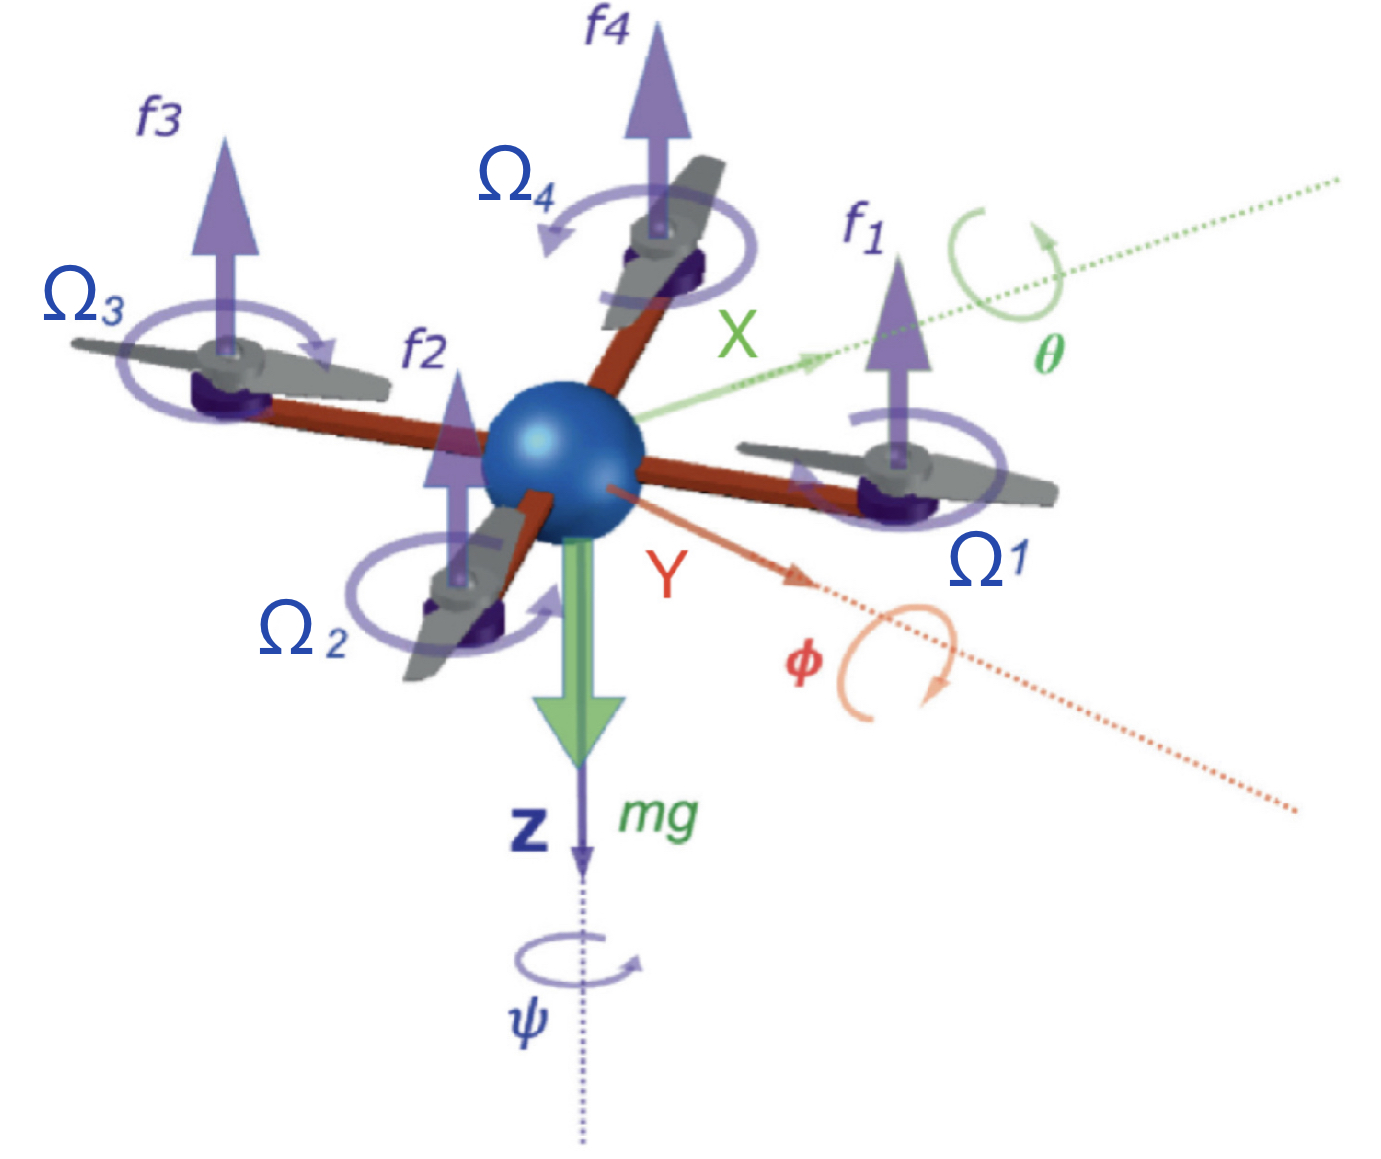
\includegraphics[width=0.5\textwidth]{gfx/quad_model}
    \caption[Modello fisico del quadrirotore, con velocità angolari dei rotori.]{Modello fisico del quadrirotore, dove $\Omega_i$ e $f_i $ ($i = 1,2,3,4$) sono rispettivamente le velocità angolari dei rotori e le relative forze di spinta generate.}
    \label{fig:quadModel}
\end{figure}

Si definiscono quattro vettori tridimensionali per rappresentare i dodici stati del modello. I primi due vettori sono definiti rispetto al sistema di riferimento \emph{mondo} ($E$) e rappresentano rispettivamente il vettore di posizione che identifica la posizione del drone nello spazio (\ref{statePos}) e il vettore di assetto che descrive (secondo gli angoli di Eulero) come il drone è ruotato intorno agli assi coordinati (\ref{stateEul}).

\begin{equation}
\Gamma_E = \begin{bmatrix}
x & y & z 
\end{bmatrix}^\top
\label{statePos}
\end{equation}

\begin{equation}
\Theta_E = \begin{bmatrix}
\phi & \theta & \psi
\end{bmatrix}^\top
\label{stateEul}
\end{equation}

I restanti vettori sono definiti rispetto al sistema di riferimento \emph{drone} ($B$) e rappresentano rispettivamente la velocità lineare (\ref{stateVelLin}) e la velocità angolare (\ref{stateVelAng}) del quadrirotore.

\begin{equation}
V_B = \begin{bmatrix}
u & v & w
\end{bmatrix}^\top
\label{stateVelLin}
\end{equation}

\begin{equation}
\omega_B = \begin{bmatrix}
p & q & r 
\end{bmatrix}^\top
\label{stateVelAng}
\end{equation}

Il moto di traslazione del velivolo è definito dall'equazione \ref{eqSist1} seguente, che mette in relazione $\Gamma_E$ e $V_B$ tramite la matrice $R_{BE}$ (\acs{DCM} definita dalla \ref{dcmBE}). 

\begin{equation}
	\dt{\Gamma_E} = R_{BE}V_B
	\label{eqSist1}
\end{equation}

Il moto di rotazione, invece, mette in relazione $\Theta_E$ e $\omega_B$. In questo caso entra in gioco una nuova matrice $J$ che consente di trasformare le variazioni degli angoli di Eulero intorno ai rispettivi assi ($\dt{\phi}, \dt{\theta}, \dt{\psi}$) nel vettore di velocità angolare del quadrirotore $\omega_B$, come mostra l'equazione \ref{jacobian}.

\begin{equation}
	J\dt{\Theta_E} = \omega_B
	\label{jacobian}
\end{equation}

Considerando la matrice inversa (\ref{invJacobian}) si ottiene l'equazione del moto di rotazione cercata (\ref{eqSist2}).

\begin{equation}
	\dt{\Theta_E} = J^{-1}\omega_B
	\label{eqSist2}
\end{equation}

\begin{equation}
J^{-1}
=
\begin{bmatrix}
1 & \sin(\phi)\tan(\theta) & \cos(\phi)\tan(\theta)\\
0 & \cos(\phi) & -\sin(\phi)\\
0 & \frac{\sin(\phi)}{\sin(\theta)} & \frac{\cos(\phi)}{\cos(\theta)}
\end{bmatrix}
\label{invJacobian}
\end{equation}\\

Prima di poter formulare il modello matematico del quadrirotore è necessario fare un'ipotesi semplificativa. Ogni sistema rotante, infatti, risente del cosiddetto effetto giroscopico, cioè un fenomeno che tende a mantenere il sistema sul suo asse di rotazione. Risulta quindi più difficile cambiare l’assetto, ma siccome l’effetto è tanto più forte quanto più la velocità di rotazione è grande, e in questo caso non ci sono grandi velocità, l’effetto è trascurabile. Si può dimostrare che trascurandolo, il modello può essere quindi scritto con il seguente sistema di equazioni nel sistema di riferimento \emph{drone}.

\begin{equation}
	\begin{cases}
	\Dot{u} = (vr - wq) + g\sin((\theta) \\
	\Dot{v} = (wp - ur) - g\cos(\theta)\sin(\phi) \\
	\Dot{w} = (uq - vp) - g\cos(\theta)\sin(\phi) + \frac{U_1}{m} \\
	\Dot{p} = \frac{I_{YY} - I_{ZZ}}{I_{XX}}qr + \frac{U_2}{I_{XX}} \\
	\Dot{q} = \frac{I_{ZZ} - I_{XX}}{I_{YY}}pr + \frac{U_3}{I_{YY}} \\
	\Dot{r} = \frac{I_{XX} - I_{YY}}{I_{ZZ}}pq + \frac{U_4}{I_{ZZ}}
	\end{cases}
	\label{modelloQuadrirotoreDrone}
\end{equation}

Dove i termini $U_i$ ($i = 1,2,3,4$) sono i termini di controllo del quadrirotore e sono infatti definiti in funzione delle velocità angolari dei rotori $\Omega_i$ ($i = 1,2,3,4$), come mostra la \ref{defControls}.

\begin{equation}
	\begin{cases}
	U_1 = b({\Omega_1}^2 + {\Omega_2}^2 + {\Omega_3}^2 + {\Omega_4}^2) \\
	U_2 = lb(- {\Omega_2}^2 + {\Omega_4}^2) \\
	U_3 = lb(- {\Omega_1}^2 + {\Omega_3}^2) \\
	U_4 = d(- {\Omega_1}^2 + {\Omega_2}^2 - {\Omega_3}^2 + {\Omega_4}^2)
	\end{cases}
	\label{defControls}
\end{equation}

Inoltre, nel modello (\ref{modelloQuadrirotoreDrone}) sono presenti i termini $I_{XX}, I_{YY}, I_{ZZ}$, cioè gli elementi diagonali della matrice di inerzia $I$, indicata nella \ref{matInerzia}. Quest'ultima risulta diagonale perché per ipotesi l'origine del sistema di riferimento del drone è nel suo centro di massa e gli assi corrispondono agli assi principali di inerzia.
 
\begin{equation}
I =
\begin{bmatrix}
I_{XX} & 0 & 0\\
0 & I_{YY} & 0\\
0 & 0 & I_{ZZ}
\end{bmatrix}
\label{matInerzia}
\end{equation}

Infine, vale la pena spiegare il significato dei coefficienti $b$ e $d$, che legano le velocità angolari dei rotori ai termini di controllo.\\

Il termine $b$ è il cosiddetto coefficiente di thrust. È un coefficiente che lega la spinta alla velocità angolare secondo la seguente equazione.

\begin{equation}
	b = \frac{T}{\Omega^2}
	\label{thrustCoeff}
\end{equation}

Dove $\Omega$ è la velocità di un generico rotore e $T$ è la spinta che genera verso l'alto. Si misura in $[N s^2]$ ed è considerato costante e uguale per tutti i rotori. La spinta verso l'altro è pertanto descritta dal termine di controllo $U_1$ nella \ref{defControls}.\\

Il termine $d$ è il cosiddetto coefficiente di drag. Quando le pale di un rotore girano in un certo verso, nasce una forza dovuta alla resistenza del vento nel senso opposto che genera un momento. Nella dinamica del quadrirotore, il coefficiente $d$ incide sull'angolo di imbardata, legato alla variazione dei momenti. Anche questo coefficiente è considerato costante e uguale per tutti i rotori, si misura in $[N m s^2]$ ed è definito come segue:

\begin{equation}
	d = \frac{Q}{\Omega^2}
\end{equation}

dove $Q$ è il momento della forza di trascinamento. Nella \ref{defControls} il termine $U_4$ tiene conto di questo contributo.\\

Poi, i termini $U_2$ e $U_3$ sono legati rispettivamente agli angoli di roll e pitch. Nello specifico, $U_2$ è legato alla differenza delle spinte date dai rotori di indice due e quattro, cioè (dalla \ref{thrustCoeff}) ai prodotti $b{\Omega_2}^2$ e $b{\Omega_4}^2$, poi moltiplicata per il braccio $l$. Analogo è il discorso per $U_3$, ma chiaramente interessa i rotori di indice uno e tre.\\

Si può anche scrivere il modello dinamico riferito al sistema \emph{mondo} tramite il sistema di equazioni definito nella \ref{modelloQuadrirotoreMondo}.

\begin{equation}
	\begin{cases}
	\Ddot{X} = (sin(\psi)sin(\phi) + cos(\psi)sin(\theta)cos(\phi))\frac{U_1}{m} \\
	\Ddot{Y} = (-cos(\psi)sin(\phi) + sin(\psi)sin(\theta)cos(\phi))\frac{U_1}{m} \\
	\Ddot{Z} = -g + (cos(\theta)cos(\phi))\frac{U_1}{m} \\
	\Dot{\phi} = p + sin(\phi)tan(\theta)q + cos(\phi)tan(\theta)r \\
	\Dot{\theta} = cos(\phi)q + cos(\theta)sin(\phi)r \\
	\Dot{\psi} = -sin(\phi)q + cos(\theta)cos(\phi)r
	\end{cases}
	\label{modelloQuadrirotoreMondo}
\end{equation}

Si nota facilmente che il modello dinamico ottenuto (definito dalla \ref{modelloQuadrirotoreDrone} nel sistema solidale al drone e dalla \ref{modelloQuadrirotoreMondo} nel sistema solidale alla terra) è di tipo non lineare.

% ------------------------------ QUATERNIONI ------------------------------

\section{Angoli di Eulero e Quaternioni}
Come spiegato nel paragrafo precedente, ogni rotazione di un corpo rigido può essere descritta mediante i tre angli di Eulero, che specificano una sequenza di tre rotazioni successive intorno agli assi coordinati. Da un lato questa rappresentazione risulta facile da comprendere e, dal punto di vista dell'implementazione, necessita semplicemente di tre numeri reali floating point. Dall'altro soffre il problema del gimbal lock (o blocco cardanico).\\

\subsection{Gimbal Lock}
Si tratta di un fenomeno problematico dei giroscopi causato dall'allineamento di due assi rotanti verso la stessa direzione. Il blocco causa la perdita del grado di libertà corrispondente all'asse bloccato.\\

Nello specifico, il problema si verifica quando il valore di alcuni angoli raggiunge valori critici. Infatti, se ad esempio il valore dell'angolo di pitch ($\theta$) dovesse raggiungere i 90 gradi, il sensore a bordo del velivolo non sarebbe in grado di distinguere tra roll ($\phi$) e yaw ($\psi$). Osservando la Figura \ref{fig:gimbal_lock} si nota come l'orientazione relativa al caso B possa essere frutto di due rotazioni differenti: un beccheggio seguito da un rollio oppure un'imbardata seguita da un beccheggio.

\begin{figure}[H]
    \centering
    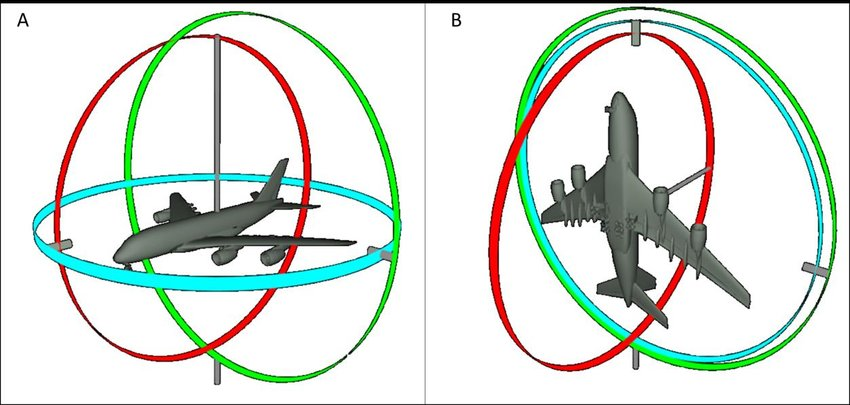
\includegraphics[width=0.7\textwidth]{gfx/gimbal_lock}
    \caption[Problema del blocco cardanico.]{Problema del blocco cardanico. Caso A: non si verifica il blocco cardanico. Caso B: rollio (roll) e imbardata (yaw) sono bloccati e risultano indistinguibili, quindi si perde un grado di libertà (blocco cardanico).}
    \label{fig:gimbal_lock}
\end{figure}

Questa problematica si riscontra facilmente anche nel modello matematico. Infatti, osservando la matrice $T$ che descrive il moto rotazionale del quadrirotore, si nota come per $\theta = \pm 90 \deg$ questa risulta singolare (determinante nullo).\\

Esistono due metodi differenti per risolvere questo problema. Il primo prevede semplicemente di utilizzare gli angoli di Eulero ad una condizione: gli angoli misurati dai sensori devono mantenersi piccoli. Il secondo, molto utilizzato, consiste nell'utilizzo dei quaternioni.

\subsection{Quaternioni}
Introdotto da William Rowan Hamilton nel 1843 come estensione dei numeri complessi, un quaternione è un elemento scrivibile come:
\[ a + bi + cj + dk \]
dove $a, b, c, d$ sono numeri reali e $i, j, k$ si comportano in modo simile all'unità immaginaria dei numeri complessi. Si può dire che la prima coordinata $a$ costituisce la parte scalare o reale del quaternione, mentre le rimanenti tre coordinate $b, c, d$ ne costituiscono la parte vettoriale o immaginaria.\\

\pagebreak

Pertanto, un quaternione è identificato da quattro numeri reali e può essere scritto come un vettore di $\mathbb{R}^4$ come segue.
\[
q = \begin{bmatrix}
q_0 & q_1 & q_2 & q_3
\end{bmatrix}^\top
\]
con $q_0, q_1, q_2, q_3 \in \mathbb{R}$.\\

Un quaternione unitario è un quaternione di norma unitaria.
\[ || q || = q_0^2 + q_1^2 + q_2^2 + q_3^2 = 1 \]

La totalità dei quaternioni unitari forma una ipersfera quadrimensionale in $\mathbb{R}^4$.
\[ S^3 = \{ (q_0, q_1, q_2, q_3) \in \mathbb{R}^4 | q_0^2 + q_1^2 + q_2^2 + q_3^2 = 1\} \]

 Questi particolari quaternioni possono essere utilizzati per descrivere l'assetto del quadrirotore nel sistema di riferimento \acs{ABC} rispetto al sistema di riferimento inerziale fisso \cite{quatAndRot}.

\begin{figure}[H]
    \centering
    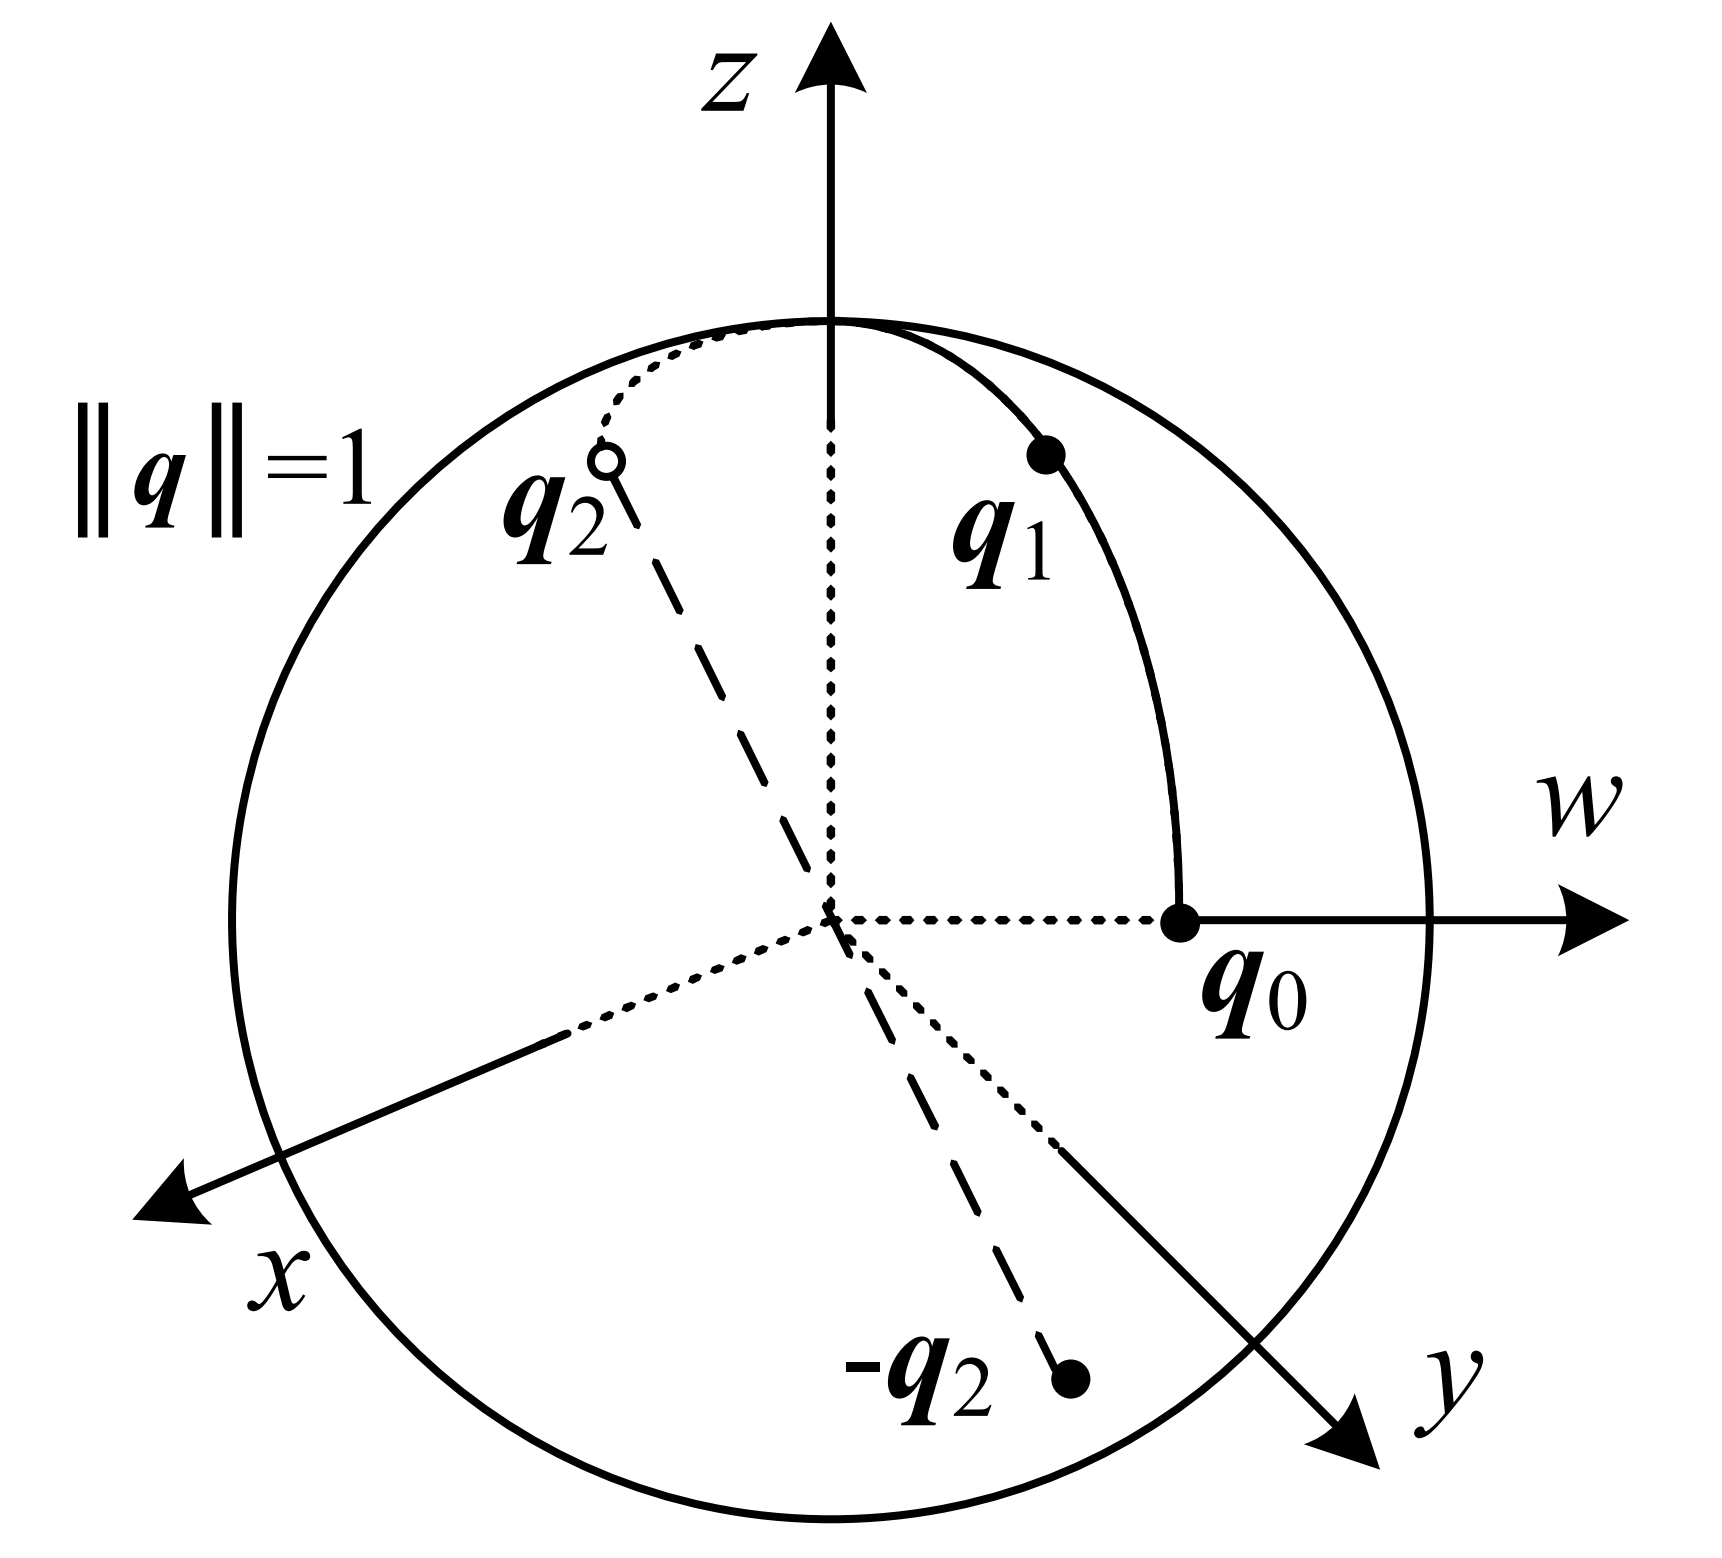
\includegraphics[width=0.4\textwidth]{gfx/quaternion}
    \caption[Rappresentazione grafica di una rotazione tramite un quaternione unitario.]{Rappresentazione grafica di una rotazione tramite un quaternione unitario.}
    \label{fig:quat}
\end{figure}

Somma e prodotto di due quaternioni sono definiti tenendo conto delle relazioni fondamentali\footnote{William Rowan Hamilton scrisse per la prima volta questa formula il 16 Ottobre 1843 camminando lungo il Broom Bridge, che attraversa il Royal Canal, a Cabra, Dublino, Irlanda. Tale evento è ad oggi commemorato da una targa collocata sul ponte che recita: "Mentre qui passeggiava, il 16 ottobre 1843 Sir William Rowan Hamilton, in un lampo d'ispirazione scoprì la formula fondamentale per la moltiplicazione dei quaternioni (\ref{hamiltonQuat}) e la incise su una pietra di questo ponte."}:
\begin{equation}
	 i^2 = j^2 = k^2 = ijk = -1
	 \label{hamiltonQuat}
\end{equation}

Le relazioni che legano gli angoli di Eulero ($\phi, \theta, \psi$) al quaternione unitario ($q$) corrispondente sono mostrate nelle equazioni \ref{quatEul} e \ref{eulQuat}.

\begin{equation}
	\begin{cases}
		q_0 = c(\frac{\phi}{2})c(\frac{\theta}{2})c(\frac{\psi}{2}) + s(\frac{\phi}{2})s(\frac{\theta}{2})s(\frac{\psi}{2}) \\
		q_1 = s(\frac{\phi}{2})c(\frac{\theta}{2})c(\frac{\psi}{2}) - c(\frac{\phi}{2})s(\frac{\theta}{2})s(\frac{\psi}{2}) \\
		q_2 = c(\frac{\phi}{2})s(\frac{\theta}{2})c(\frac{\psi}{2}) + s(\frac{\phi}{2})c(\frac{\theta}{2})s(\frac{\psi}{2}) \\
		q_3 = c(\frac{\phi}{2})c(\frac{\theta}{2})s(\frac{\psi}{2}) - s(\frac{\phi}{2})s(\frac{\theta}{2})c(\frac{\psi}{2})
	\end{cases}
	\label{quatEul}
\end{equation}

\begin{equation}
	\begin{cases}
		\phi = \tan^{-1} \left[\frac{2(q_2q_3 + q_0q_1)}{q_0^2 - q_1^2 - q_2^2 + q_3^2}\right] \\
		\theta = \sin^{-1} \left[-2(q_1q_3 + q_0q_2)\right] \\
		\psi = \tan^{-1} \left[\frac{2(q_1q_2 + q_0q_3)}{q_0^2 + q_1^2 - q_2^2 - q_3^2}\right]
	\end{cases}
	\label{eulQuat}
\end{equation}\\

Come detto, questa soluzione è ampiamente utilizzata in ambito informatico e robotico. Infatti, molti linguaggi di programmazione e molte librerie forniscono direttamente operazioni di conversione tra angoli di Eulero e quaternioni unitari, come si vedrà nel seguito.

% ------------------------------ CONTROLLO ------------------------------

\section{Controllo di un Quadrirotore}
Un quadrirotore a X presenta quattro rotori posizionati come in Figura \ref{fig:quadRotors}. Essendo i motori e le eliche sullo stesso piano, è necessario equilibrare il moto del drone impiegando due motori che ruotano in senso orario e due che ruotano in senso antiorario. Nello specifico, i rotori M1 e M4 ruotano in senso orario (clockwise o CW), mentre i rotori M2 e M3 ruotano in senso antiorario (counterclockwise o CCW). Questa contrapposizione permette di annullare l'energia rotatoria dei motori e quindi eventuali coppie di reazione.

\begin{figure}[H]
    \centering
    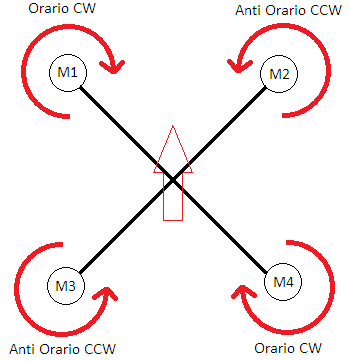
\includegraphics[width=0.3\textwidth]{gfx/rotori_quadrotor}
    \caption[Funzionamento dei rotori di un quadrirotore a X.]{Disposizione e funzionamento dei rotori di un quadrirotore con eliche disposte a X.}
    \label{fig:quadRotors}
\end{figure}

\subsection{Manovre di Spinta, Rollio, Beccheggio e Imbardata}

Nel seguito si descrive il funzionamento delle quattro principali manovre di controllo del quadrirotore. Tre di queste manovre sono dovute al cambiamento dell'assetto del drone nel tempo, cioè alle variazioni degli angoli di Eulero (rollio, beccheggio e imbardata). È possibile alterare questi angoli modificando le velocità dei quattro rotori in modo specifico. La quarta e ultima manovra di controllo, invece, riguarda la spinta del quadrirotore verso l'alto, mantenendone fisso l'assetto.

\section*{Manovra di Spinta}
Quando il vettore di spinta (thrust) è allineato alla verticale (direzione ortogonale al piano individuato dal quadrirotore) e ha modulo maggiore della forza peso del drone ($F_p = mg$ dove $m$ è la massa del drone e $g$ è l'accelerazione gravitazionale), si verifica una traslazione verticale lungo l'asse Z. Come specifica la relazione \ref{thrustCoeff}, la spinta generata è legata al quadrato delle velocità angolari dei rotori. In condizioni di equilibrio statico (hovering) ciascun rotore genera una spinta pari ad un quarto della forza peso del drone. Per aumentare il modulo della spinta verso l'alto (asse Z positivo) si aumentano le velocità di tutti i rotori di una stessa quantità, in modo da non creare differenze che possano modificare l'assetto del drone. In Figura \ref{fig:thrust_quad} è mostrato il concetto.

\begin{figure}[H]
    \centering
    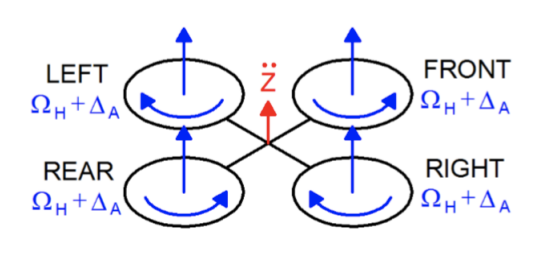
\includegraphics[width=0.5\textwidth]{gfx/thrust_quad}
    \caption[Manovra di spinta di un quadrirotore.]{Manovra di spinta: la velocità di tutti i rotori aumenta di una quantità costante.}
    \label{fig:thrust_quad}
\end{figure}

\section*{Manovra di Rollio}
Il rollio contribuisce allo spostamento del drone lungo l'asse Y (destra e sinistra). Si ottiene lasciando invariate le velocità dei motori anteriore (FRONT) e posteriore (REAR), e cambiando di una certa quantità le velocità dei motori di destra (RIGHT) e sinistra (LEFT); come mostrato in Figura \ref{fig:roll_quad}.

\begin{figure}[H]
    \centering
    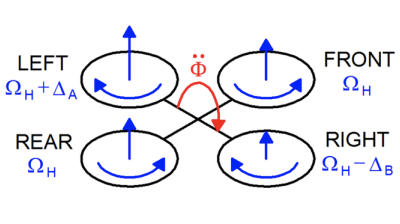
\includegraphics[width=0.39\textwidth]{gfx/roll_quad}
    \caption[Manovra di rollio di un quadrirotore.]{Manovra di rollio: cambia la velocità dei rotori di destra (RIGHT) e sinistra (LEFT).}
    \label{fig:roll_quad}
\end{figure}

\section*{Manovra di Beccheggio}
Il beccheggio contribuisce allo spostamento del drone lungo l'asse X (avanti e indietro). Si ottiene, analogamente al rollio, lasciando invariate le velocità dei motori di destra (RIGHT) e sinistra (LEFT), e cambiando di una certa quantità le velocità dei motori anteriore (FRONT) e posteriore (REAR); come mostrato in Figura \ref{fig:pitch_quad}.

\begin{figure}[H]
    \centering
    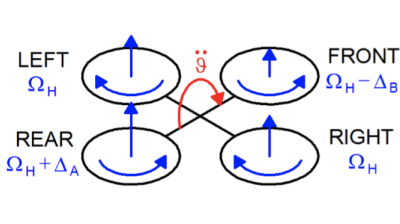
\includegraphics[width=0.39\textwidth]{gfx/pitch_quad}
    \caption[Manovra di beccheggio di un quadrirotore.]{Manovra di beccheggio: cambia la velocità dei rotori anteriore (FRONT) e posteriore (REAR).}
    \label{fig:pitch_quad}
\end{figure}

\section*{Manovra di Imbardata}
L'imbardata è il movimento più complesso. L’idea fondamentale è cambiare il momento rispetto all’asse z, immaginato uscente dal piano dei rotori, e mantenere costante la spinta verso l’alto. Per ottenere questo, si aumenta la velocità dei rotori di due motori opposti, e si diminuisce la velocità dei due restanti rotori. In questo modo si avranno, per esempio, due rotori che girano velocemente in senso orario, e due che girano più lentamente in senso antiorario. Nel complesso ci sarà dunque un momento che fa girare il drone intorno all’asse z. Se le velocità sono opportunamente scelte, non ci sarà un cambiamento della spinta verso l’alto. La Figura \ref{fig:yaw_quad} riassume quanto detto.

\begin{figure}[H]
    \centering
    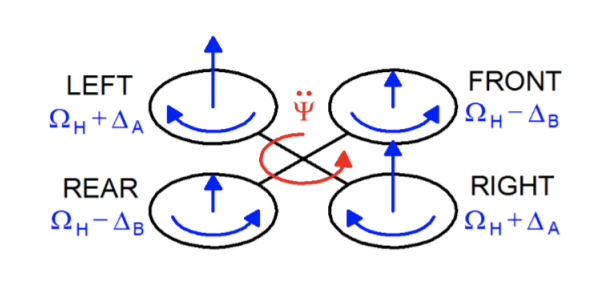
\includegraphics[width=0.47\textwidth]{gfx/yaw_quad}
    \caption[Manovra di imbardata di un quadrirotorre.]{Manovra di imbardata.}
    \label{fig:yaw_quad}
\end{figure}

\subsection{Controllo Stabilizzato e Acrobatico}
Esistono due modalità di volo e quindi di controllo di un quadrirotore. La modalità stabilizzata, anche nota come self-level, e la modalità acrobatica, anche nota come rates e utilizzata per droni da gara.\\

Nel primo caso si controlla il drone agendo sugli angoli di Eulero, come esposto nel paragrafo precedente. Nel secondo caso, invece, il segnale di controllo inviato al drone non contiene gli angoli di Eulero, ma le velocità angolari. Questo significa che, controllando il drone ad esempio con un radiocomando e lasciando andare le levette di roll e pitch verso il centro (cioè portandole a zero), nel primo caso il velivolo ritorna in posizione neutrale (piana ed allineata con l'orizzonte), mentre nel secondo caso si mantiene l'angolo di rotazione sugli assi di roll e pitch impostati.
